\def\name{MLMC for Uncertainty Quantification in Reservoir Simulation}

\begin{frame}{\name{}}
    \setlength{\cw}{0.6\textwidth}%
    \begin{overlayarea}{\textwidth}{\frameheight}
        \vspace{2em}
        \begin{columns}
            \begin{column}{\cw}
                \begin{squarelist}
                    \item<1-> Incompressible flow in porous media \visible<4->{-- \redtext{SPDE}}
                    \only<1>{%
                        \begin{align*}
                            \vel(\vx) = -\perm(\vx)\nabla p(\vx), \quad \nabla \cdot \vel(\vx) =  q(\vx)
                        \end{align*}
                    }%
                    \only<2-3>{%
                        \begin{align*}
                            -\nabla \cdot \big(\perm(\vx)\nabla p(\vx)\big) = q(\vx)
                        \end{align*}
                    }%
                    \only<4->{%
                        \begin{align*}
                            -\nabla \cdot \big(\perm(\vx, \redtext{\omega})\nabla p(\vx, \redtext{\omega})\big) = q(\vx,\redtext{\omega})
                        \end{align*}
                    }%
                    \item<3-> Permeability $\perm$ is \emph{uncertain}
                    \begin{vertlist}
                        \item Few physical samples, uncertain seismic data
                    \end{vertlist}
                    \item<4-> Modelled as random field $K(\vx, \redtext{\omega})$
                    \begin{vertlist}
                        \item Spatial \emph{and} stochastic variable $(\vx, \redtext{\omega}) \in \spa \times \Omega$
                    \end{vertlist}
                    \item<5-> Fixing $\redtext{\omega}$ gives a deterministic PDE
                \end{squarelist}
            \end{column}
            \begin{column}{0.95\textwidth - \cw}
                \only<1-3>{%
                    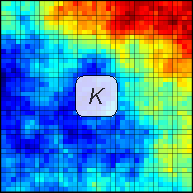
\includegraphics[width = \textwidth]{figures/perm/perm.pdf}
                }%
                \only<4->{%
                    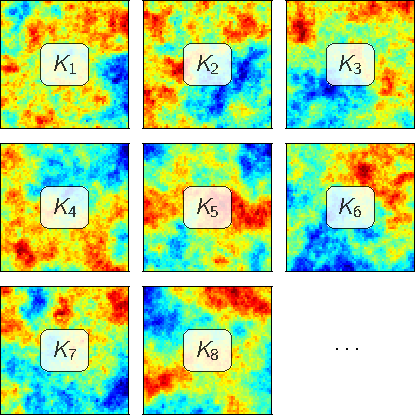
\includegraphics[width = \textwidth]{figures/perm/perm-samples.pdf}
                }%
            \end{column}
        \end{columns}
    \end{overlayarea}
\end{frame}

\begin{frame}{\name{}}
    \setlength{\cw}{0.6\textwidth}%
    \def\dx{1.5em}%
    \begin{overlayarea}{\textwidth}{\frameheight}
        \vspace{1em}%
        \textbf{Two-phase flow in porous media}
        \begin{align*}
            \partial_t(\phi S_\alpha) + \nabla \cdot \vel_\alpha = q_\alpha, \quad  \vel_\alpha = -\lambda_\alpha\perm\nabla p, \quad \alpha = w, o
        \end{align*}
        \vspace{-1.7em}
        \begin{block}{}
            \small
            \begin{center}
                $\phi$: porosity \hspace{\dx} $S_\alpha$: saturation \hspace{\dx} $\vel_\alpha$: Darcy velocity \hspace{\dx} $q_\alpha$: sources/sinks \hspace{\dx} $\lambda_\alpha$: mobility
            \end{center}
        \end{block}
        \vspace{0.3em}
        \begin{squarelist}
            \item<2-> Quantity of interest $\un$ typically derived from simulation results\only<2>{, e.g.}
            \only<2>{%
                \begin{center}
                    \small%
                    \begin{tabular}{l|l}
                        Saturation at time $t'$ & $\un = S_w(\vx, t')$ \\
                        Water production rate & $\un = q_w(t)$\\
                        Total oil production & $\un = Q_o$
                    \end{tabular}
                \end{center}
            }%
            \only<3->{\\... which are all random variables}
        \end{squarelist}
        \vspace{0.5em}
        \only<3->{
            \begin{figure}
                \centering
                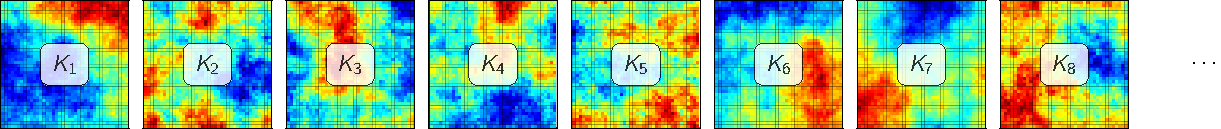
\includegraphics[width = \textwidth]{figures/perm/perm-samples-row.pdf}
            \end{figure}
        }
    \end{overlayarea}
\end{frame}

\begin{frame}{\name{}}
    \begin{overlayarea}{\textwidth}{\frameheight}
        \vspace{1em}
        \begin{squarelist}
            \item<1-> Quantity of interest $\un$ generally not scalar, but defined over domain $\Lambda$
            \begin{center}
                \small%
                \begin{tabular}{l|l|l}
                    Saturation at time $t'$ & $\un = S_w(\vx, t')$ & $\Lambda = D$ (physical domain)\\
                    Water production rate & $\un = q_w(t)$ & $\Lambda = [0,T]$ (time domain) \\
                    Total oil production & $\un = Q_o$ & $\Lambda$ not applicable
                \end{tabular}
            \end{center}
            \vspace{0.5em}
            \item<2-> Necessary substitutions with appropriate norm \redtext{$\|\cdot\|$} over $\Lambda$
            \begin{equation*}
                |\expect[\un_\ell] - \expect[\un]| \rightarrow \redtext{\|}\expect[\un_\ell] - \expect[\un]\redtext{\|}, \quad \var[\expecta_\ell] \rightarrow \expect\left[\redtext{\|}\expecta_\ell - \expect[\expecta_\ell]\redtext{\|}^2\right]
            \end{equation*}
            \item<3-> Most of the theory for scalar variables follows directly -- particularly with \redtext{$L^2(\Lambda)$-norm}:
            \begin{equation*}
                \var\big[\expecta(\un_\nlev)\big] = \sum_{\ell = 0}^\nlev \frac{\vara_\ell}{\nsamp_\ell}, \quad \text{where } \vara_\ell = \expect\left[\redtext{\|}\expecta_\ell - \expect[\expecta_\ell]\redtext{\|}^2\right]
            \end{equation*}
        \end{squarelist}
    \end{overlayarea}
\end{frame}

\begin{frame}{\name{}}
    \renewcommand{\thealgocf}{}
    \only<1-4>{%
        \begin{algorithm}[H]
            \caption*{Multilevel Monte Carlo Method}
            \only<3>{\graytext}{%
                \textbf{Input:} Hierarchy of approximations $\ell = 0, \dots, \nlev$, tolerance $\tol$ \\
                \For(\tcp*[f]{Warmup}){$\ell = 0, \dots, \nlev$}{
                    Compute $\nsamp_w$ samples of $\un_\ell - \un_{\ell-1}$\tcp*[r]{Local MC}
                }
                Estimate $\vara_\ell$, $\cost_\ell$ and optimal $\nsamp_w = \nsamp_\ell + \nsamp_\ell'$ given desired tolerance $\tol$\\
            }%
            \only<2>{\graytext}{%
                \While(\tcp*[f]{Multilevel MC}){any extra samples needed, ($\nsamp_\ell' > 0$)}{
                    \For{$\ell = 0, \dots, \nlev$}{
                        Compute $\nsamp_\ell'$ more samples of $\un_\ell - \un_{\ell-1}$\tcp*[r]{Local MC}
                    }
                    Update estimates $\vara_\ell$, $\cost_\ell$ and optimal $\nsamp_\ell = \nsamp_\ell + \nsamp_\ell'$ given desired accuracy $\tol$ \\
                }
            }%
        \end{algorithm}
    }%
\end{frame}